\documentclass{scrbook}

\usepackage{polyglossia}
\usepackage{amssymb}
\usepackage{amsthm}
\usepackage{amsmath}
\usepackage{minted}
\usepackage{xcolor}
\usepackage[autostyle]{csquotes}

\DeclareQuoteAlias{german}{slovene}
\setdefaultlanguage{slovene}
\definecolor{LightGray}{gray}{0.9}

\author{ACM priprave na tekmovanja}
\date{Različica z dne \today}

\newcommand{\naslov}[1]{\section{#1}}
\newcommand{\podnaslov}[1]{\subsection{#1}}

\newcommand{\koda}[1]{\mintinline{c++}{#1}}

\newenvironment{blokkode}
{
  \begin{minted}
	[
	frame=lines,
	framesep=2mm,
	baselinestretch=1,
	bgcolor=LightGray,
	mathescape,
	linenos
	]
	{c++}
}
{
  \end{minted}
}

\newcommand{\fkoda}[1]{
  \inputminted
  [
  frame=lines,
  framesep=2mm,
  baselinestretch=1,
  bgcolor=LightGray,
  mathescape,
  linenos
  ]{c++}{#1}
}

\newcommand{\poglavje}[1]{
  \chapter{#1}
}

\title{Zapiski za tekmovalno programiranje}

\begin{document}

\maketitle

\tableofcontents
\newpage

\poglavje{Vhod in izhod}

\naslov{Osnovna struktura programa}

Programi za svoje delovanje potrebujejo način za komunikacijo z uporabnikom.
Kompleksnejši programi v ta namen uporabljajo ekran, miško in tipkovnico, pri
tekmovalnem programiranju pa najpogosteje uporabljamo najpreprostejši način za
komunikacijo: pisanje in branje s \emph{standardnega vhoda in izhoda}.
Običajno to pomeni, da se nam ob zagonu programa odpre okno, kamor lahko pišemo
programu in kamor program izpisuje stvari.
Ko želimo, da naš program kaj izpiše, uporabimo \emph{funkcijo} \koda{printf}.
Poglejmo si enostaven primer.

\fkoda{poglavja/vhod-in-izhod/helloworld.cpp}

Funkciji \koda{printf} v dvojnih narekovajih damo besedilo ali števila, ki jih
želimo izpisati.
Na koncu tega besedila napišemo \verb+\n+, ki označuje, da mora program na tem
mestu iti v novo vrstico.
To je pomembno vključiti predvsem, če funkcijo \koda{printf} uporabimo večkrat
zaporedoma, saj bi bilo sicer celotno besedilo izpisano v eni vrstici.

Posvetimo se tudi splošni obliki zgornje kode, saj vsebuje ključne elemente, ki
jih mora vsebovati vsak program.
Prva vrstica, \verb+#include <stdio.h>+, pove programu, da bomo uporabljali
funkcije za vhod in izhod, konkretno \koda{printf} in kasneje \koda{scanf}.
Če te vrstice nebi napisali, bi ob poskusu izvajanja kode sistem javil napako,
in trdil, da funkcije \koda{printf} ne pozna.

Besedilo \koda{int main()} računalniku pove, da bodo sledili zaviti oklepaji (to
so oklepaji, ki izgledajo \{takole\}), znotraj katerih bo glavno telo naše kode.
Zaenkrat bomo vso našo kodo napisali med te zavite oklepaje, ko pa bomo spoznali
sezname in kasneje funkcije, bomo nekaj kode vnesli tudi drugam.
Koda v \koda{main} je organizirana v vrstice, ki se morajo končati s podpičjem
\verb+;+.
Ko se bo program izvedel, se bodo zaporedoma od zgoraj navzdol izvedle vse
vrstice, dokler ne pridemo do zadnje vrstice, ki se mora začeti z ukazom
\koda{return}.
Temu ukazu sledi številka --- ta pove, če se je med izvajanjem programa zgodila
kakšna napaka.
Če je številka enaka $0$, se je program končal brez napak, drugim številkam pa
pravimo \emph{kode napake}.
Te so uporabne predvsem zato, da lahko uporabnik programerju le z eno številko
pove, kakšna napaka se je v programu zgodila.
Mi bomo v prihodnje večinoma pisali programe, katerih uporabniki bomo sami, zato
bomo vedno uporabili kodo $0$.

V program lahko dodamo \emph{komentarje}.
To je besedilo, ki je sicer napisano v kodi programa, a ne vpliva na njegov
potek, ker računalnik komentarjev ne izvede.
Zaradi tega lahko komentarji vsebujejo tudi besedilo v naravnem jeziku
(slovenščini), ki programerjem razlaga pomen kode poleg komentarja.
Na voljo imamo dve vrsti komentarjev:
\begin{itemize}
\item Če na začetku vrstice napišemo dve poševnici, \verb+//+, s tem dobimo
  komentar, ki prikriva besedilo v tej vrstici.
  Če se ta komentar pojavi sredi vrstice, bo prikril vse besedilo od tam naprej
  do konca vrstice.
\item Če v besedilu zapišemo poševnico in zvezdico, \verb+/*+, s tem dobimo
  komentar, ki prikriva vso besedilo do vključno prve pojavitve nasprotnega
  simbola, \verb+*/+.
\end{itemize}

\fkoda{poglavja/vhod-in-izhod/komentarji.cpp}

\naslov{Branje podatkov}

Programu lahko sporočimo različne podatke, program pa mora te podatke nekam
shraniti, preden jih lahko obravnava.
Mestu, kamor podatke shranimo, pravimo \emph{spremenljivka}, saj lahko te
podatke med tekom programa spreminjamo.
Vsem spremenljivkam v programu damo ime, s katerim se na njih sklicujemo, ter
\emph{podatkovni tip}, ki pove, kakšni podatki so v spremenljivki shranjeni
(npr.~besedilo, številka, \ldots).
V spodnjem primeru ustvarimo eno spremenljivko, ki jo imenujemo
\koda{tvoje_ime}, njen tip pa je \enquote{besedilo dolžine največ $50$}.

\fkoda{poglavja/vhod-in-izhod/branje.cpp}

Tudi \koda{scanf} je funkcija, ki ji podamo dva ali več \emph{parametrov}.
Prvi parameter mora vedno biti niz znotraj narekovajev, ki opisuje, kakšnega
tipa so podatki, ki naj jih funkcija prebere.
Ta opis podamo s \emph{formatnikom}, v zgornjem primeru \verb+%s+ računalniku
pove, da bo program prebral eno besedo.
Preostali parametri povedo, v katero spremenljivko naj funkcija shrani prebrane
podatke.
Če imamo v nizu več formatnikov, moramo podati eno spremenljivko za vsak
formatnik.

Do zdaj smo funkciji \koda{printf} podali samo točno določeno besedilo, ki smo
ga želeli izpisati.
Izpisujemo pa lahko tudi spremenljivke, kot smo to naredili v tem zadnjem
primeru.
Znotraj besedila dodamo formatnike na mesta, kjer želimo, da so spremenljivke,
potem pa izven narekovajev naštejemo imena spremenljivk, ki jih želimo izpisati.

V zgornjem primeru smo brali in izpisali niz besedila, kar pa je pravzaprav
zahtevnejše od branja in pisanja števil.
Za delo z nizi potrebujemo kompleksnejše ukaze, ki jih bomo spoznali kasneje,
zato se bomo do nadaljnjega omejili na delo s (celimi) števili.
Tem pripada tip \koda{int} (angl.~\textit{integer}) ter formatnik \verb+%d+,
kakor vidimo v naslednjem primeru.

\fkoda{poglavja/vhod-in-izhod/branje-stevil.cpp}

Pri branju števil imamo le eno dodatno zahtevo kot pri branju nizov --- pred ime
spremenljivke moramo zapisati znak \verb+&+.
Razlog za tem bomo spoznali, ko bomo obravnavali kazalce, za sedaj pa to vzemimo
kot zahtevo postopka.
Pri številih tudi ne povemo direktno največje dolžine, kakor smo to naredili pri
nizih, saj je največja velikost določena že vnaprej.
Tip \koda{int} lahko shrani pozitivna in negativna števila velikosti največ 2
milijardi.

% LocalWords:  formatnikov formatnik formatnikom formatnike


\poglavje{Računske operacije}
\naslov{Seštevanje, odštevanje in množenje}

Najpreprostejše računske operacije na številih, ki jih lahko z računalnikom
izračunamo, so seštevanje, odštevanje in množenje.
Račune zapisujemo tako kot v šoli, z \emph{operatorji}.
Za seštevanje uporabimo \koda{+}, za odštevanje \koda{-} in za množenje \koda{*}.
Poglejmo si preprost primer, kjer račun izvedemo kar v funkciji \koda{printf}.

\fkoda{poglavja/racunske-operacije/sestevanje.cpp}

Zgornji program preprosto izpiše številko $12$, ki je rezultat računa $5 + 7$.
Namesto izpisovanja lahko rezultat tudi shranimo v spremenljivko:

\fkoda{poglavja/racunske-operacije/nova-spremenljivka.cpp}

Če v ta program podamo vhod \verb+3 7+, bo izpisal tri števila: $12$, $-4$ in
$21$.
Drugo izpisano število ima pred seboj minus.
Če te to preseneča in še ne poznaš negativnih števil, si preberi naslednji
razdelek, sicer pa ga lahko izpustiš.

\podnaslov{Negativna števila}

Na meteorološki postaji Kredarica so leta 2014 izmerili povprečno januarsko
temperaturo približno \SI{-5}{\celsius}, povprečno avgustovsko pa približno
\SI{6}{\celsius}.
Med tema meritvama je \SI{11}{\celsius} razlike.
Pozimi lahko izmerimo temperature manjše od 0.
Takšnim številom, kot je $-5$, rečemo \emph{negativna števila}.
Lahko pa jih uporabimo tudi drugje, ne samo pri merjenju temperature.
S pozitivnimi števili lahko štejemo od $0$ do neskončno ($1, 2, 3, \ldots$), z
negativnimi pa do negativne neskončnosti ($-1, -2, -3, \ldots$).
Tako kot pozitivna števila jih lahko seštevamo in odštevamo:
\begin{gather*}
  5 - 11 = -6 \\
  -6 + 11 = 5 \\
  5 -(-6) = 11 \\
  -2 - 1 = -3 \\
  -2 - (-1) = -1 \\
  -2 + (-1) = -3 \\
\end{gather*}
Pri tem se sklicujemo na naslednji pravili, kjer smo z $x$ označili poljubno
število:
\begin{gather*}
  -(-x) = x \\
  +(-x) = -x
\end{gather*}
Z negativnimi števili lahko tudi množimo:
\begin{gather*}
  2 \cdot (-5) = -10 \\
  (-5) \cdot (-5) = 25
\end{gather*}
Pri tem uporabimo enostavno pravilo: številski del rezultata je enak, kot če bi
množili števili brez predznaka \verb+-+.
Če smo množili eno pozitivno in negativno število, rezultatu pripišemo še
negativni predznak, če pa smo množili dve negativni števili ali dve pozitivni
števili, pa tega ne storimo.
Računalnik pri računanju ne razlikuje med pozitivnimi in negativnimi števili,
računske operacije pišemo enako kot pri pozitivnih.

\naslov{Deljenje}

Števila lahko tudi delimo, za kar uporabimo znak \koda{/}.
Pri tem pa moramo biti pozorni, ker se deljenje v računalniku obnaša drugače kot
smo navajeni iz matematike.
Običajno pri deljenju dveh števil, recimo $3$ in $7$, dobimo ulomek:
\[
  3 / 7 = \frac{3}{7}.
\]
Če pa v C++ program zapišemo \verb+printf("%d\n", 3/7)+, bomo dobili
nepričakovan odgovor --- $0$.
To je zato, ker je deljenje v C++ \emph{celoštevilsko}.

Za lažje razumevanje si bomo pomagali s formulo $a = k \cdot b + o$, ki
ponazarja deljenje z ostankom.
Če želimo število $a$ deliti s številom $b$, bomo kot odgovor dobili dve
števili: celi del, ki smo ga uspešno delili, in ostanek, kjer deljenje ni bilo
uspešno.
Celi del smo zgoraj označili s $k$, ostanek pa z $o$.
Ko uporabimo operator \koda{/}, dobimo največje tako število, za katero je
produkt rezultata in delitelja (števila na desni strani \koda{/}) manjši ali
enak deljencu (številu na levi strani \koda{/}).
Z drugimi besedami, dobimo $k$ iz zgornjega zapisa.
Če želimo preveriti še vrednost ostanka $o$, jo lahko izračunamo iz ostalih
števil,
\[
  o = a - k \cdot b,
\]
ali pa uporabimo poseben operator \verb+%+, ki mu pravimo \emph{modulo}.
Poglejmo si, kako deljenje deluje v praksi.

\fkoda{poglavja/racunske-operacije/deljenje.cpp}

Če v zgornji program vpišemo dve števili, bo izpisal rezultat deljenja ter
razcep števila po zgornji formuli.
Na primer, ob vhodu \verb+25 7+ dobimo naslednji izpis:
\begin{verbatim}
rezultat deljenja je 3, z ostankom 4
25 = 3 * 7 + 4
\end{verbatim}
če pa vpišemo \verb+3 7+, dobimo
\begin{verbatim}
rezultat deljenja je 0, z ostankom 3
3 = 0 * 7 + 3
\end{verbatim}
Kaj pa se zgodi, če vpišemo \verb+5 0+?
V tem primeru bo program poskusil deliti z $0$, kar v matematiki (in v
programiranju) ni dovoljeno.
Program se bo zato sesul in ne bo izpisal ničesar, odvisno od našega
operacijskega sistema pa morda dobimo kakšno sporočilo o napaki.
Ko delimo ali računamo ostanek z modulom, in je število na desni strani
operatorja spremenljivka, katere vrednosti ne poznamo vnaprej, moramo preveriti,
če je slučajno enaka $0$.
Če je, operacije ne smemo izvesti!

\poglavje{Pogojni stavki}
Pogosto želimo, da računalnik izvaja drugačno kodo glede na vrednost ene ali
več spremenljivk, npr.~da nam pokaže drugačno vsebino, če smo napisali
pravilno ali napačno geslo, da računalo sešteva, če smo pritisnili gumb za
seštevanje, oz.~odšteva, če smo pritisnili gumb za odštevanje.
Z drugimi besedami, želimo upravljati potek programa (torej izbrati, katera koda
naj se izvede) glede na vrednosti spremenljivk.
Angleško takemu upravljanju pravimo \emph{control flow}, najpogosteje pa ga
izvajamo s t.i.~\emph{pogojnimi stavki}.
Osnovna struktura je sledeča:

\fkoda{poglavja/pogojni-stavki/sintaksa.cpp}

\emph{Pogoj} je nov pojem. Označuje neke vrste račun, katerega rezultat ni
število, vendar \emph{logična vrednost}.
Tu sta možni vrednosti le dve: pravilno (angl.~\koda{true}) in napačno
(angl.~\koda{false}).
Če bo rezultat računa, navedenega v običajnih oklepajih v zgornjem \koda{if}
stavku, \koda{true}, se bo izvedla koda znotraj prvih zavitih oklepajev, če pa
je rezultat računa \koda{false}, pa se bo izvedla koda v drugih zavitih
oklepajih (tistih za besedo \koda{else}).
Drugega dela, tj.~\koda{else} in oklepaje za njim, ni treba pisati, če tega ne
želimo.

Kako pa zapišemo pogoj?
Za to uporabimo posebne \emph{logične operatorje}.
Pri delu s številkami so nam na voljo naslednji:
\begin{itemize}
\item \koda{==}: primerja dve številski vrednosti.
  Rezultat je \koda{true}, če sta vrednosti enaki.
\item \koda{!=}: primerja dve številski vrednosti.
  Rezultat je \koda{true}, če sta vrednosti različni.
\item \koda{<}: primerja dve številski vrednosti.
  Rezultat je \koda{true}, če je vrednost na levi manjša od vrednosti na desni.
\item \koda{>}: deluje podobno kot \koda{<}, le da v drugo smer;
  rezultat je \koda{true}, če je vrednost na desni manjša od vrednosti na levi.
\item \koda{<=}: primerja dve številski vrednosti.
  Rezultat je \koda{true}, če sta vrednosti enaki, ali če je vrednost
  na levi manjša od vrednosti na desni.
\item \koda{>=} deluje podobno kot \koda{<=}, le da v drugo smer.
\end{itemize}

Poglejmo si primer uporabe pogojnega stavka.

\fkoda{poglavja/pogojni-stavki/stevila.cpp}

Program v zgornjem primeru primerja dve števili z vsemi naštetimi operatorji.
Če v program vpišemo npr.~števili $3$ in $7$, vstopimo v drugi, tretji in peti
pogojni stavek, zaradi česar se izpišejo naslednje vrstice:
%
\begin{verbatim}
Stevili sta razlicni.
Prvo stevilo je manjse od drugega.
Prvo stevilo je manjse ali enako drugemu.
\end{verbatim}
%
Če pa v program dvakrat vnesemo število $12$ (ali katerokoli drugo število), pa
dobimo naslednji izhod:
%
\begin{verbatim}
Stevili sta enaki.
Prvo stevilo je manjse ali enako drugemu.
Prvo stevilo je vecje ali enako drugemu.
\end{verbatim}

Pozorni moramo biti, da pri primerjavi enakosti dveh števil napišemo dva
enačaja, \koda{==}.
Če zapišemo le en enačaj, kot v matematiki (torej \koda{=}), se bo program sicer
zagnal, vendar ne bo deloval pravilno.
Enojnega enačaja nikoli ne uporabljamo v pogoju \koda{if} stavka!

Oglejmo si še primer uporabe stavka \koda{else}.
Spodnji program bo uporabnika vprašal za PIN, in mu napisal, če je bil PIN
pravilen oziroma napačen.

\fkoda{poglavja/pogojni-stavki/pin.cpp}

Pogojne stavke lahko tudi gnezdimo, torej vstavimo enega v drugega.
Spodnji program od uporabnika sprejme naročilo v restavraciji, kjer ponujajo
dve vrsti hrane; juhe in sendviče.
Na voljo sta dve vrsti juhe, in dve vrsti sendvičev.
Za izbiro kosila uporabnik prvo izbere med juho in sendvičem, nato pa še okus.

\fkoda{poglavja/pogojni-stavki/nesting.cpp}

Pozorni bodimo na postavitev kode.
Običajno kodo znotraj zavitih oklepajev \koda{if} stavka pišemo tako, da je
poravnana štiri presledke bolj desno od kode zunaj \koda{if} stavka.
V nekaterih programskih jezikih je taka poravnava obvezna, v C/C++ pa ne, vendar
nezamaknjena koda že v majhnih programih postane popolnoma nepregledna.
Branje in popravljanje kode je veliko lažje, če del kode znotraj zavitih
oklepajev zamaknemo za štiri presledke.
Za to lahko uporabimo tudi tipko Tab, ki se na tipkovnici nahaja levo od tipke
Q.
Kode kot spodaj nikoli ne pišemo!

\fkoda{poglavja/pogojni-stavki/unindented.cpp}

% LocalWords:  nezamaknjena


\poglavje{Zanke}
\naslov{Sintaksa}

V programiranju pogosto želimo nek del kode ponoviti, zato uporabljamo
\emph{zanke}.
Poznamo več zank, a najpogosteje uporabljamo zanko \koda{for}.
Le-ta ima tri posebne komponente: \emph{začetek}, \emph{pogoj} in \emph{korak}.
Poglejmo si preprost primer, ki trikrat izpiše besedo \texttt{nekaj}.

\fkoda{poglavja/zanke/sintaksa.cpp}

Poglejmo si, kako ta program deluje. Podpičja v peti vrstici razdelijo okrogle
oklepaje na tri dele: začetek (\koda{int stevec=0}), pogoj (\koda{stevec < 3})
in korak (\koda{stevec++}).
Začetek se bo izvedel, ko se ta zanka začne.
Vsakič preden se izvede koda v notranjosti zanke, se preveri pogoj.
Če pogoj drži, se bo izvedla koda v zanki, sicer pa se bo zanka končala.
Korak je podoben začetku, in se izvede na koncu vsake ponovitve zanke.

V zgornjem primeru začetek naredi novo številko \koda{stevec} in jo nastavi na
$0$.
Pogoj preveri, če je \koda{stevec} manjši od $3$, korak \koda{stevec++} pa je
okrajšava za \koda{stevec = stevec + 1}, torej poveča \koda{stevec} za $1$.
Program sledi naslednjem postopku:
\begin{enumerate}
	\item Program se začne in pride do for zanke,
	  najprej se izvede začetek \koda{int stevec=0}.
	\item Zdaj se je začela zanka, preveri se pogoj \koda{stevec < 3}.
	  Ker je \koda{stevec} za zdaj še $0$, je pogoj izpolnjen.
	  Izvede se vsebina zanke, torej program izpiše \texttt{nekaj}.
	  Zdaj smo prišli do konca zanke, izvede se korak, zato se \koda{stevec}
	  poveča na $1$, program pa skoči nazaj na začetek zanke.
	\item Ker smo na začetku zanke, se preveri pogoj, \koda{stevec < 3},
	  \koda{stevec} je zdaj $1$ in je pogoj še vedno izpolnjen, zato se izvede
	  vsebina zanke.
	  Ko program še enkrat izpiše \texttt{nekaj}, izvede korak, \koda{stevec}
	  poveča na $2$ in skoči nazaj na začetek.
	\item Spet smo na začetku, zato se preveri pogoj, \koda{stevec} je zdaj $2$,
	  kar je manjše od $3$, zato se \texttt{nekaj} izpiše še tretjič.
	  Program potem poveča \koda{stevec} na $3$ in skoči nazaj na začetek.
	\item Ker smo spet na začetku, se bo še enkrat preveril pogoj,
	  a zdaj je \koda{stevec} enak $3$ in $3$ ni manjše od $3$,
	  zato se zanka konča.
	  Ker je naslednji ukaz \koda{return 0}, se bo program tam končal.
\end{enumerate}
%
Vredno je omeniti, da je naš števec zavzel vrednosti $0$, $1$, in $2$, kar se
morda zdi čudno, glede na to, da bi ponavadi šteli do tri kot $1,2,3$.
Tovrstno štetje od nič je zelo pogosto v programiranju, in bo prišlo prav
kasneje, ko se bomo učili o seznamih.

\naslov{Primeri uporabe}

\podnaslov{Spreminjanje dolžine zanke}

Zanka, ki smo jo napisali zgoraj, se bo vedno ponovila trikrat.
Kaj pa če hočemo, da se zanka ponovi glede na neko število na vhodu?
Seveda je tudi to mogoče in sicer tako, da vstavimo našo spremenljivko v pogoj
zanke.
Poglejmo si primer.

\fkoda{poglavja/zanke/puscica.cpp}

Zgornji program sprejme število in nariše puščico te dolžine.
Tu uporabimo še en trik, in sicer v funkciji \koda{printf} znotraj zanke ne
dodamo \verb+\n+, s čimer dosežemo to, da so v izhodu znaki \verb+-+ eden zraven
drugega v isti vrstici in ne vsak v svoji.

\podnaslov{Branje števil v zanki}

Ena od moči računalnikov je zelo hitra obdelava velike količine podatkov,
računalnik bo na primer zlahka seštel tisoč števil, medtem ko bi bilo to početi
na roke precej zamudno.
Poglejmo si, kako bi napisali program, ki bi nekaj izračunal z več števili.

\fkoda{poglavja/zanke/branje-stevil.cpp}

V zgornjem primeru prvo preberemo število \koda{n}, nato pa ustvarimo
spremenljivko \koda{vsota}, ki jo takoj nastavimo na $0$.
V tej spremenljivki bomo hranili vsoto števil, ki smo jih do sedaj videli
na vhodu (razen \koda{n}), na koncu programa bo torej enaka vsoti vseh takih
števil.

Opazimo, da v zanki namesto \koda{stevec} sedaj uporabljamo \koda{i}, ki je
tradicionalna izbira za spremenljivko v zanki.
V notranjosti zanke so zdaj trije ukazi.
Najprej naredimo novo spremenljivko, ki jo poimenujemo \koda{sestevanec} in
preberemo naslednje število iz vhoda.
Nato pa z okrajšavo \koda{vsota += sestevanec} prištejemo spremenljivki
\koda{vsota} spremenljivko \koda{sestevanec}.
Na daljše bi to lahko napisali kot \koda{vsota = vsota + sestevanec}.
V vsaki iteraciji tako prištejemo ravno prebrano število k vsoti, na koncu pa
bomo izpisali vsoto vseh.

\podnaslov{Zanka z drugačnim korakom in začetkom}

Do zdaj so vse naše zanke takole:
\koda{for (int i=0; i < 10; i++)}, torej so začele z nič in se nekajkrat
ponovile.
C++ pa nam dovoli, da lahko z našimi zankami naredimo veliko več.
Kot primer si poglejmo zanko, ki izpiše vsa soda števila med $1$ in $100$.

Pozorno poglejmo števila, ki jih moramo izpisati.
Ker $1$ ni sodo, bo prvo izpisano število $2$.
Število $3$ prav tako ni sodo, tako da bomo izpisali $4$, po tem pa $6$, $8$,
$10$ in tako dalje.
Vidimo, da vsak korak povečamo izpisano število za $2$, napišimo torej program.

\fkoda{poglavja/zanke/soda-stevila.cpp}

Ker se želena števila začnejo z dva, bomo v začetni del zanke vpisali
\koda{int i=2}.
Ker želimo izpisati števila med $1$ in $100$ in ne med $1$ in $99$, bomo v
pogojnem delu uporabili znak manjše ali enako, \koda{i<=100}
(pogoj \koda{i<100} ne bi veljal za število $100$).
Ker želimo povečati naše število za $2$ vsak korak, smo v polje za korak
napisali \koda{i += 2}.
Edina stvar, ki jo naredimo v notranjosti napisane zanke pa je, da izpišemo
trenutno vrednost spremenljivke \koda{i}.

\poglavje{Seznami}
\naslov{Sintaksa}

Ko si želimo podatke shraniti tako, da jih bomo lahko spreminjali in na koncu
nekaj z njimi naredili (npr.~da z njimi računamo, jih izpišemo, itd.), za to
uporabimo spremenljivke.
Vsaka spremenljivka hrani en podatek -- vse spremenljivke do sedaj so hranile le
eno številko.
Pogosto pa si želimo števila shraniti tako, da bomo kasneje lahko dostopali do
njih, ampak med pisanjem programa ne vemo točno, s koliko števili bo program
moral delati.
Problem rešimo s seznami.

Da ustvarimo seznam (angl.~\emph{array}), zapišemo tip spremenljivke, ki ga bodo
imeli vsi elementi seznama (trenutno poznamo le \koda{int}, a bomo kmalu
spoznali tudi druge tipe spremenljivk), nato seznamu damo ime, in na koncu v
oglatih oklepajih zapišemo dolžino seznama, takole:

\fkoda{poglavja/seznami/sintaksa.cpp}

Tukaj smo ustvarili seznam z imenom \koda{seznam_stevil}, ki hrani $300$ števil.
Če želimo dostopati do elementov seznama, ali nastaviti njihove vrednosti, tudi
uporabimo oglate oklepaje, kot v spodnjem primeru.

\fkoda{poglavja/seznami/dostopanje.cpp}

Tu smo prvo nastavili tretji element seznama na $7$, nato smo nastavili četrti
element seznama na $9$, in za tem nastavili peti element seznama na njuno vsoto.
Ostalih elementov seznama se nismo dotaknili.
Tako kot pri spremenljivkah nismo smeli uporabiti vrednosti spremenljivke,
preden smo ji vrednost nastavili, moramo paziti, da vrednosti posamičnega
elementa seznama ne uporabljamo, preden je ne nastavimo.
Narobe bi bilo na primer izpisati \koda{seznam_stevil[2]} ali to vrednost
uporabiti v računu, saj je nismo nikoli nastavili.

Pri dostopanju do elementov seznama moramo paziti tudi na naslednje dejstvo:
če imamo seznam dolžine $N$, potem so elementi tega seznama oštevilčeni s
številkami od $0$ do $N-1$ vključno, ne pa s številkami od $1$ do $N$, kot bi
morda pričakovali.
V zgornjem primeru tako lahko zapišemo \koda{seznam_stevil[0]},
\koda{seznam_stevil[1]}, \ldots, \koda{seznam_stevil[299]}, ne pa tudi
\koda{seznam_stevil[300]}.
Pravimo, da so seznami \emph{indeksirani} od $0$ naprej.

Poglejmo si primer preproste naloge.
Na vhodu je podano število $N$, ki mu sledi $N$ števil.
Program mora izpisati ta števila (razen prvega, $N$), v obratnem vrstnem redu.
V ta namen ustvarimo seznam z imenom \koda{seznam}, ki lahko shrani največ
$1000$ (predpostavimo, da uporabnik ne bo vnesel več kot $1000$ števil).
Potem s \koda{for} zanko preberemo $N$ števil in vsako shranimo v svoj element
seznama, začenši z $0$.
Na koncu se s še eno \koda{for} zanko sprehodimo skozi $i = 0, 1, \ldots, N-1$.
Na vsakem koraku izračunamo indeks (položaj) elementa, ki je $i$-ti od konca
seznama, in ga shranimo v spremenljivko \koda{obratni}.
Ta indeks je natanko \koda{N-i-1}, saj mora za \koda{i=0} biti
\koda{obratni=N-1}, za \koda{i=1} mora biti \koda{obratni=N-2}, itd.
Da se seznam na izhodu izpiše v obratnem vrstnem redu, preprosto izpišemo
\koda{seznam[obratni]}.

\fkoda{poglavja/seznami/obrni.cpp}

Poglejmo si še malo bolj zanimiv primer.
Naša naloga sedaj je, da uredimo seznam $N$ števil ($N \le 10^6$) po velikosti
od najmanjšega do največjega.
Podano imamo tudi informacijo, da bodo ta števila velika med vključno $0$ in
$100$.
Naloge se lahko lotimo tako, da preštejemo, kolikokrat se neko število pojavi v
danem seznamu, nato pa bomo seznam rekonstruirali tako, da bo urejen.
Da preštejemo, kolikokrat se kakšno število pojavi, uporabimo nov seznam, kjer
indeks pomeni številko, ki jo štejemo, shranjena vrednost pa kolikokrat smo to
številko že prešteli.

\fkoda{poglavja/seznami/counting.cpp}

Ta algoritem za urejanje je zelo znan; imenuje se urejanje s preštevanjem
(angl.~\emph{counting sort}).
Primeren je, kadar imamo zelo majhen razpon možnih vrednosti števil, kakor smo
imeli tu ($0 - 100$).
Obstajajo tudi drugi algoritmi za urejanje.
Nekatere bomo spoznali kasneje.

\podnaslov{Večdimenzionalni seznami}

Videli smo, kako ustvariti seznam števil, kaj pa seznam seznamov?
Takemu seznamu pravimo \emph{dvodimenzionalen seznam}, ustvarimo pa ga tako,
da napišemo dva zaporedna oglata oklepaja z velikostjo, kot spodaj:

\fkoda{poglavja/seznami/sintaksa-2d.cpp}

Dvodimenzionalni seznami so uporabni, kadar moramo podatke predstaviti v tabeli.
Do posamičnih elementov dostopamo z dvojnimi oglatimi oklepaji, tako kot pri
inicializaciji spremenljivke; \koda{tabela[i][j]}.
Tabele si običajno predstavljamo tako, da nam prvi indeks poda zaporedno
številko vrstice, drugi pa zaporedno številko stolpca.
Sicer pa z njimi delamo enako kot z običajnimi seznami.

\poglavje{Nizi in besedilo}
Poleg dela s številkami od računalnika pogosto želimo, da nekaj naredi z nizi
besedila.
Primeri takšnih programov so npr.~urejevalniki besedila, ki jih uporabljamo tako
za pisanje \enquote{enostavnega} besedila (kode), kot tudi za razna obogatena
besedila.
Pravzaprav pa skoraj vsak računalniški program dela z besedilom; kadarkoli
želimo uporabniku prikazati neke informacije, jih moramo namreč izpisati na
zaslon.
Ko smo delali s številkami, smo problem izpisovanja prepustili računalniku, ker
je kodo za branje in izpisovanje številk k sreči napisal že nekdo drug.
Za pisanje splošnih programov pa tovrstno znanje ne bo dovolj, zato si poglejmo
osnove dela z besedili.

Pri slovenščini se naučimo, da je besedilo sestavljeno iz več odstavkov,
odstavek iz več povedi, poved iz več stavkov, stavek iz več besed, besede pa iz
več črk.
Pri tem se moramo zavedati, da stavke ločimo z ločili (vejice, pike, klicaji,
itd.), besede ločimo s presledki, posamične odstavke pa ločimo z zamikanjem prve
povedi v desno.
Za predstavitev v računalniku je tak model preveč zakompliciran, zato vzamemo
bolj enostavnega.
Besedila bomo predstavili z \emph{nizi} (angl.~\emph{string}), ki bodo
zaporedja več \emph{znakov} (angl.~\emph{character}).
Vse, kar bi si kadarkoli zaželeli izpisati, bomo proglasili za znak.
Tako si bomo vse črke predstavljali kot znak, kjer bomo ločili tudi med velikimi
in malimi črkami (saj vendar izgledajo drugače, če jih napišemo), prav tako bomo
za znake proglasili tudi ločila, oklepaje in matematične operacije
(\verb|+, -, *, /|).
Poleg tega bomo za znak proglasili tudi števke od 0 do 9, ker tudi njih
izpišemo (večje številke pa so sestavljene iz teh števk, zato ne potrebujemo
posebnih znakov za njih).

Nenazadnje bomo ustvarili še nekaj posebnih znakov, ki jih morda nebi
pričakovali.
Od teh bomo zdaj spoznali tri: znak za presledek, znak za novo vrstico in znak
za konec besedila.
Znak za presledek bomo uporabili, kjerkoli želimo imeti prostor med dvema
besedama (torej presledek).
Za razliko od slovenščine tudi presledke obravnavamo, kot da bi bili pravzaprav
neke posebne črke.
Znak za novo vrstico bomo uporabili tam, kjer želimo, da izpis našega programa
skoči vrstico nižje; brez tega znaka nam bo program vse izpisal v eni zelo dolgi
vrstici besedila.
Ta znak označimo s posebno kodo \verb+\n+ (ker se v angleščini ta znak imenuje
\emph{new line}), opazimo pa, da ga v funkciji \koda{printf} uporabljamo že od
prvega programa, ki smo ga napisali.
Uporabili bomo tudi znak za konec besedila, ki ga označimo z \verb+\0+,
pogosto pa mu rečemo tudi \emph{NULL}.
Več o temu znaku bomo povedali kasneje.

\naslov{Predstavitev znakov}

Preden si pogledamo nize, moramo razumeti, kako delamo z znaki.
V C++-u imamo za to poseben tip \koda{char}, ki nam hrani en znak.
Če želimo spremenljivki tipa \koda{char} nastaviti vrednost, moramo želeni znak
dati v enojne narekovaje, kot spodaj:

\fkoda{poglavja/nizi/basic-char-syntax.cpp}

S to kodo ustvarimo spremenljivko tipa \koda{char}, ki hrani vrednost
\koda{'A'}, torej znak za veliko črko A.
Tako kot števila lahko tudi znake pišemo in beremo; pri tem uporabimo
\koda{printf} s formatnikom \verb+%c+, narejen za znake.

\fkoda{poglavja/nizi/scanf-printf-char.cpp}

\begin{table}[h!]
  \centering
  \begin{tabular}[h!]{|c|c|}
	\hline
	Znak & ASCII koda \\
	\hline
	NULL (\verb+\0+) & 0 \\
	Nova vrstica (\verb+\n+) & 10 \\
	Presledek (\verb+' '+) & 32 \\
	\hline
	\verb+0+ & 48 \\
	\verb+1+ & 49 \\
	\verb+2+ & 50 \\
	\vdots & \vdots \\
	\verb+9+ & 57 \\
	\hline
	\verb+A+ & 65 \\
	\verb+B+ & 66 \\
	\verb+C+ & 67 \\
	\vdots & \vdots \\
	\verb+Z+ & 90 \\
	\hline
	\verb+a+ & 97 \\
	\verb+b+ & 98 \\
	\verb+c+ & 99 \\
	\vdots & \vdots \\
	\verb+z+ & 122 \\
	\hline
  \end{tabular}
  \caption{Del ASCII tabele}%
  \label{tab:ascii}
\end{table}

Ker so računalniki narejeni za delo s številkami, moramo tudi znake
predstaviti kot številke.
To dosežemo s t.i.~\emph{kodnimi tabelami}, ki vsakemu znaku priredijo eno
številko.
Najpreprostejša kodna tabela je ASCII, ki lahko zakodira vse črke angleške
abecede ter vse ostale zgoraj naštete znake, ne zmore pa zakodirati šumnikov ali
večine črk, ki se ne pojavljajo v angleški abecedi.
Prav zaradi tega razloga se pri programiranju takih črk izogibamo, kar se le da.
ASCII kode nekaterih pogostih znakov so prikazane v tabeli~\ref{tab:ascii}.
Opazimo lahko, da so števke in črke v tabeli zaporedno; števka \verb+0+ ima kodo
48, števka \verb+1+ 49, \ldots, črka \verb+A+ ima kodo 65, \verb+B+ ima kodo 66,
itd.
Opazimo tudi, da so velike črke od malih ločene, in da imajo male črke večje
kode.

Ta dejstva lahko uporabimo v programih tako, da črke preprosto obravnavamo, kot
da bi bile številke.
Črki \koda{'a'} lahko npr.~prištejemo neko številko, in tako dobimo črko, ki je
toliko znakov naprej v abecedi; \koda{'a' + 7} je na primer enako \koda{'h'}.
Poleg tega lahko znake med sabo primerjamo, kar bomo videli v prvem primeru.

Poglejmo si spodnji primer, kjer je prikazano, kako na enostaven način
preverimo, ali je neka črka velika ali majhna.
Koda sprva prebere eno črko iz vhoda, nato pa preveri, če je vpisana črka med
\koda{A} in \koda{Z}; če ni, potem preverimo še, ali je črka med \koda{a} in
\koda{z}.

\fkoda{poglavja/nizi/is-capital-letter.cpp}

Če dobro pogledamo v tabelo, vidimo, da koda $0$ ne pripada števki \koda{0}, pač
pa znaku za konec besedila.
To se morda na prvi pogled zdi nepričakovano, ampak ima svoj smisel; če je
števka del besedila, o njej ne razmišljamo kot o številki, temveč pač o nekem
znaku, ki ima v drugem kontekstu drugačen pomen.
Če želimo to števko pretvoriti v številko, s katero lahko brez skrbi računamo,
lahko uporabimo trik, kjer \enquote{odštejemo nič}, kot spodaj:

\fkoda{poglavja/nizi/odstevanje-nic.cpp}

Pri tem triku moramo biti previdni, da odštejemo pravilno ničlo; če odštejemo
številko $0$, se ne bo nič spremenilo; tako kot pri matematiki namreč
odštevanje ničle številke ne spremeni.
Če pa odštejemo \emph{znak} \koda{'0'} (v enojnih narekovajih), pa dejansko
odštevamo številko $48$, tj.~ASCII kodo znaka \koda{'0'}.
Praktično uporabo tega trika bomo pokazali v naslednjem razdelku.

\naslov{Predstavitev nizov}

Niz predstavimo kot seznam znakov, ki ga pišemo podobno kot seznam številk:

\fkoda{poglavja/nizi/basic-string-syntax.cpp}

Ta ukaz pove računalniku, naj ustvari spremenljivko z imenom
\koda{niz_besedila}, ki hrani \emph{največ} $300$ znakov.
V tej spremenljivki bomo hranili naše zaporedje besedila.
Če želimo nize brati ali pisati, uporabimo funkciji, ki ju že poznamo, ter
formatnik \verb+%s+, tu pa je ena posebnost; za branje nizov pred imenom
spremenljivke \underline{ne} zapišemo znaka \verb+&+, kakor to zapišemo za
branje številk ali znakov.
Če želimo neko spremenljivko nastaviti na niz, ki ga ne bomo prebrali, jo lahko
nastavimo na običajen način z enačajem, ter z dvojnimi narekovaji.
Tak način podajanja nizov smo že srečali; namreč vedno, ko uporabimo funkciji
\koda{scanf} ali \koda{printf}.

Poglejmo si preprost primer uporabe.
Spodnji program prebere uporabnikovo ime in ga pozdravi.

\fkoda{poglavja/nizi/pozdravljen.cpp}

Ko ustvarimo niz, računalniku povemo, kolikšna je njegova najdaljša možna
dolžina.
Nič pa nam ne preprečuje, da v to spremenljivko shranimo krajši niz.
Kako pa potem računalnik ve, kje se naš niz dejansko konča?
Pričakujemo namreč, da bomo za zapis kratkega niza uporabili nekaj mest za znake
na začetku, potem pa se bo niz nekje končal; kaj je na neuporabljenih mestih
zaporedja, nas ne zanima.
Ravno iz tega razloga so nizi zgrajeni tako, da imajo na koncu dodaten znak, ki
označuje konec besedila.
To je znak NULL, ki smo ga omenili na začetku.
Ta znak pove računalniku, da se besedilo tu konča in da naj naprej ne gleda.
Če vrednost niza nastavimo z enačajem ali niz preberemo s \koda{scanf}, bo
računalnik sam poskrbel, da bo ta znak napisan na pravo mesto; če pa z nizi
delamo kaj bolj zapletenega, moramo za ta znak skrbeti sami.
Zaradi tega znaka je dejansko število vidnih znakov, ki jih lahko shranimo v
niz, za eno manjše od predpisane največje dolžine.
Da se tovrstnim problemom izognemo, bomo od sedaj naprej vedno napisali nekaj
večjo število za dolžino niza; če pričakujemo, da uporabnik vpiše največ $200$
znakov, bomo za velikost niza dejansko napisali $201$ (ali celo malo več).

Kot primer, kako uporabimo zgornje dejstvo, si poglejmo spodnji program, ki
izračuna dolžino niza.

\fkoda{poglavja/nizi/dolzina-niza.cpp}

Ta koda ni težka, vendar jo je pogosto neprijetno pisati, zato imamo boljšo
alternativo; če na začetek programa dodamo \verb+#include <string.h>+, lahko
uporabljamo funkcijo \koda{strlen}, ki nam ravno tako izračuna dolžino niza:

\fkoda{poglavja/nizi/dolzina-niza-bolje.cpp}

Funkcijo \koda{strlen} uporabljamo v skoraj vsakem programu z nizi, zato je
dobro, da se je čim prej navadimo.
Poleg tega \koda{strlen} dolžino dejansko izračuna hitreje kakor zgornja koda.

V naslednjem primeru bomo napisali kodo, ki pretvori besedilo v velike črke.
Za to uporabimo eno od lastnosti ASCII tabele, ki smo jo omenili prej; namreč,
da so črke napisane zaporedno, in da so velike črke pred malimi.

\fkoda{poglavja/nizi/upcase.cpp}

Za zadnji primer v tem razdelku si poglejmo, kako bi pretvorili številko,
zapisano z nizom, v številko, zapisano v spremenljivki tipa \koda{int}.
Prej omenjen trik z odštevanjem nič ne bo deloval, ker lahko z njim
pretvarjamo le znake; lahko pa številko pretvorimo znak po znak.
Pri tem pretvarjanju uporabljamo lastnosti desetiškega zapisa števil; namreč,
da zaporedna mesta v zapisu predstavljajo vrednosti, ki se razlikujejo za
faktor $10$.
Ko pretvorimo prvi del besedila, in želimo dopisati še eno števko, moramo že
zapisani del \enquote{premakniti} eno mesto v levo, ter premaknjenemu številu
prišteti novo števko.
Premikanje dosežemo z množenjem z $10$.

\fkoda{poglavja/nizi/string-v-stevilo.cpp}

\naslov{Standardne funkcije}

Izkaže se, da pri delu z nizi pogosto pišemo zelo podobne kose programa, kakor
se je zgodilo pri primeru z izračunom dolžine.
Namesto da večkrat napišemo skoraj enako kodo, so v knjižnici \verb+string.h+
dostopne razne funkcije, ki nam pogosto olajšajo delo.

\podnaslov{Primerjava nizov}

Za primerjavo dveh nizov \underline{ne} uporabljamo dvojnega enačaja
(\koda{==}), temveč funkcijo \koda{strcmp}.
Funkcijo uporabimo tako, da ji v okrogle oklepaje napišemo dva niza;
\koda{strcmp(niz1, niz2)}.
Če sta niza enaka, funkcija vrne rezultat \texttt{0}, sicer pa vrne drugačen
rezultat.
Spodnja koda preveri, če je uporabniku ime Filip:

\fkoda{poglavja/nizi/ali-si-filip.cpp}

Funkcija nam pravzaprav poda več informacij.
Z njo lahko pogledamo, kakšna je \emph{leksikografska ureditev} dveh nizov;
preprosto povedano, kateri od nizov bi se, če bi bila oba niza besedi, pojavil
prej v slovarju (leksikonu).
Če bi se prvi niz pojavil prej, funkcija vrne negativno število.
Če bi se drugi niz pojavil prej, pa funkcija vrne pozitivno število.

\podnaslov{Kopiranje nizov}

Če želimo eno spremenljivko prekopirati v drugo, lahko napišemo \koda{b = a}.
Na žalost pa to ne deluje za nize; namesto \koda{niz2 = niz1} moramo napisati
\koda{strcpy(niz2, niz1)}.
Funkcija \koda{strcpy} prekopira drugi niz v prvega; na koncu bosta oba niza
imela enako vsebino.

Če želimo nekemu nizu na konec dodati nek drug niz, lahko za to uporabimo
funkcijo \koda{strcat} (\emph{string concatenate}).
Ta funkcija prav tako sprejme dva niza; ko jo pokličemo, drug niz kopira na
konec prvega.

\podnaslov{Operacije na prvih $m$ znakih}

Včasih želimo kopirati ali primerjati le del niza.
Za to imamo na voljo malce drugačne verzije zgoraj naštetih funkcij; če v imenih
teh funkcij za \koda{str} dodamo še \koda{n} (torej \koda{strncmp},
\koda{strncpy}, \ldots), in funkciji kot zadnji argument podamo številko $m$, bo
funkcija svoje delo opravila le na prvih $m$ znakih;
\koda{strncmp(niz1, niz2, 3)} bo primerjal le prve tri znake,
\koda{strncpy(niz2, niz1, 7)} bo kopiral le prvih sedem znakov, ipd.

\poglavje{Vhod in izhod: dopolnitev}
\naslov{Dodatni formatniki za \texttt{scanf}}

Poleg že znanih formatnikov \verb+%d+, \verb+%lld+ in \verb+%s+ poznamo tudi
druge, ki so lahko uporabni v različnih situacijah.
Seznam pogosto uporabnih formatnikov je v
tabeli~\ref{tab:vhod-in-izhod-dopolnitev:formatniki}.
V tabeli se pojavi izraz \emph{prazen znak}, angl.~\emph{whitespace} --- to je
znak, ki zasede prostor v spominu (in kateremu pripada ASCII koda), vendar se na
zaslonu ne pojavi.
Poznamo tri take znake, to se presledek, tabulator \verb+\t+ in znak za novo
vrstico \verb+\n+.
Formatniki \verb+%d+, \verb+%lld+ in \verb+%s+ preberejo, a ignorirajo, prazne
znake, ki se pojavijo pred vsebino, ki jo formatnik dejansko shrani.
Če npr.~v spodnji primer programa vpišemo vhod
\begin{verbatim*}
Hello

   World!
\end{verbatim*}
bo program prebral le ti dve besedi, in ne praznih znakov med njima.

\begin{table}[h]
  \centering
  \begin{tabular}{c|l}
	formatnik & opis \\
	\hline
	\verb+%%+ & en znak \verb+%+ \\
	\verb+%d+ & število tipa \koda{int} \\
	\verb+%lld+ & število tipa \koda{long long} \\
	\verb+%c+ & poljuben znak (lahko tudi prazen znak) \\
	\verb+%s+ & zaporedje nepraznih znakov \\
	\verb+%[...]+ & zaporedje znakov, ki se pojavijo med oglatimi oklepaji \\
	\verb+%[^...]+ & zaporedje znakov, ki se ne pojavijo med oglatimi oklepaji
  \end{tabular}
  \caption{Različni formatniki za \koda{scanf} in \koda{printf}}%
  \label{tab:vhod-in-izhod-dopolnitev:formatniki}
\end{table}


\fkoda{poglavja/vhod-in-izhod-dopolnitev/formatnik-s.cpp}

Zadnja formatnika v tabeli, \verb+%[...]+ in \verb+%[^...]+ sta bolj zapletena
od ostalih.
Uporabljamo ju tako, da namesto tropičja v oglate oklepaje zapišemo seznam
znakov, ki so dovoljeni v prebranem besedilu.
Tako lahko npr.~enostavno ločimo besedo, sestavljeno iz črk in številk na niz in
na število, ki ga lahko takoj shranimo v \koda{int}:

\fkoda{poglavja/vhod-in-izhod-dopolnitev/primer-branje-niza-in-stevila.cpp}

Če zgornjemu programu kot vhod podamo \texttt{aacbb012}, bo izpisal
\begin{verbatim}
Niz: aacbb, stevilo: 12
\end{verbatim}
Če želimo dovoliti vse male črke abecede, lahko namesto seznama vseh črk
zapišemo tudi \verb+%[a-z]+, podobno lahko za velike črke uporabimo
\verb+%[A-Z]+, za števke pa \verb+%[0-9]+.
Formatnik bo v zadnjem primeru še vedno prebral niz znakov, in ga ne bo
avtomatsko pretvoril v \koda{int}.
Tudi te obsege lahko kombiniramo, formatnik \verb+%[a-z2-7B]+ npr.~prebere niz,
sestavljen iz malih črk angleške abecede, števk med $2$ in $7$ ter velike črke
B.

Formatnik \verb+%[^...]+ deluje podobno kot formatnik \verb+%[...]+, le da
prebere vse znake, razen tistih, ki smo jih zapisali namesto tropičja.
Ta formatnik je uporaben pri branju niza do konca vrstice, česar s formatnikom
\verb+%s+ ne moremo narediti, če nimamo podanega števila besed v vrstici.
Primer je prikazan v spodnjem programu, kjer uporabimo tudi formatnik
\verb+%*c+.
Ta deluje enako kot formatnik \verb+%c+, le da znaka, ki ga prebere, nikjer ne
shrani, zato zanj tudi ne podamo spremenljivke.
Ta formatnik je potreben, ker \verb+%[^\n]+ ne prebere znaka za novo vrstico, ki
ga \enquote{počistimo} z \verb+%*c+.
Če bi želeli prebrati dve zaporedni vrstici in nebi uporabili \verb+%*c+, nebi
druga uporaba formatnika \verb+%[^\n]+ shranila ničesar, saj bi nemudoma
naletela na znak za novo vrstico, in zaključila branje.

\fkoda{poglavja/vhod-in-izhod-dopolnitev/do-konca-vrstice.cpp}

\naslov{Neznano število podatkov}

Če vemo točno, koliko besed, številk oz.~vrstic bomo imeli na vhodu, jih lahko
preberemo z zanko.
Kaj pa, če ne vemo, koliko podatkov bo na vhodu, kot v nalogi
\putka{neznane-vsote}{Neznane vsote}?
Če podatke beremo v neskončni zanki, bomo sicer prebrali vse, a se program ne
bo nikoli ustavil.
V naslednjem primeru je nakazano, kako ta problem rešimo:

\fkoda{poglavja/vhod-in-izhod-dopolnitev/do-konca-vhoda.cpp}

Funkcija \koda{scanf} vrne število formatnikov, ki jih je uspešno prebrala (če
ji kot parameter npr.~podamo samo \verb+%d+, bo vrnila $1$, če je uspešno
prebrala število, sicer pa $0$).
Posebno vrednost \koda{EOF} (End of File) pa vrne, če na vhodu ni ničesar več za
prebrati.
Tedaj se bo zanka ustavila.
Če programu vhodne podatke podajamo iz datoteke, se to zgodi avtomatsko ob koncu
datoteke, če pa mu podatke podajamo na roko, konec vhoda sporočimo s
\verb|Ctrl+D| (Linux in MacOS) ali \verb|Ctrl+Z| (Windows).

\naslov{Uporaba nizov ali datotek za vhodno-izhodni sistem}

Včasih si lahko pri procesiranju podatkov pomagamo s tem, da dano besedilo prvo
shranimo v niz, preden ga pretvorimo v drugo obliko, ali iz njega izluščimo
podatke.
Pri tem si lahko pomagamo s funkcijama \koda{sscanf} in \koda{ssprintf}, ki
delujeta podobno kot poznana \koda{scanf} in \koda{printf}, vendar namesto
branja iz oz.~pisanja na standardni vhod oz.~izhod delujeta z nizi v spominu.
Niz, s katerega beremo oz.~na katerega pišemo, podamo kot prvi argument v ti
funkciji, kakor v spodnjem primeru.

\fkoda{poglavja/vhod-in-izhod-dopolnitev/sscanf-sprintf.cpp}

Podobno lahko s pomočjo funkcij \koda{fscanf} ter \koda{fprintf} beremo iz in
pišemo v datoteke na računalniku.
Datoteke predstavimo s posebnim tipom \koda{FILE}, pri katerem moramo poleg
imena spremenljivke napisati tudi zvezdico (zakaj je temu tako, spoznamo v enem
od kasnejših poglavij).
Da se povežemo s pravo datoteko, uporabimo funkcijo \koda{fopen}, ki ji podamo
dva argumenta.
Prvi argument je ime datoteke, ki jo želimo uporabljati, drug argument pa je
možnost odpiranja.
Za naše potrebe sta dovolj dve možnosti, \koda{"r"}, ki pove, da bomo datoteko
odprli v načinu za branje, ter \koda{"w"}, ki pove, da bomo datoteko odprli v
načinu za pisanje.
Slednja možnost tudi ustvari datoteko z danim imenom, če ta ne obstaja, oziroma
izbriše vso besedilo v tej datoteki, če datoteka že ima vsebino.
Primer uporabe funkcij \koda{fscanf} in \koda{fprintf} je prikazan spodaj.
Opazimo, da se na koncu programa pojavi tudi funkcija \koda{fclose}.
Ta funkcija operacijskemu sistemu pove, da smo z branjem oz.~pisanjem
zaključili, in da lahko spremembe na tej točki shrani v dejansko datoteko (brez
klica te funkcije shranjevanje sprememb ni zagotovljeno).
Funkcijo moramo nujno poklicati za vsako datoteko, ki smo jo odprli z
\koda{fopen}.

\fkoda{poglavja/vhod-in-izhod-dopolnitev/datoteke.cpp}

%#endblock
% LocalWords:   formatniki scanf formatnikov formatnik formatnika tropičja
% LocalWords:  formatnikom vhodno-izhodni


\poglavje{Spomin in kazalci}
\naslov{Računalniški spomin}

Spomin, pomnilnik ali angl.~RAM (\emph{Random access memory})
je ključna komponenta v računalniku. Med tekom programa so v njem shranjene vse
spremenljivke, ki jih program uporablja.
S spremenljivkami lahko naredimo tudi več, kot smo se do sedaj naučili, vendar
pa moramo za to razumeti, kako je spomin zgrajen.

Osnovna enota za merjenje količine informacij je \emph{bit}.
En bit informacij ustreza odgovoru na eno vprašanje tipa da ali ne
-- če nam nekdo pove, da so vrata zaprta, nam je podal en bit informacij,
ker so lahko vrata bodisi odprta bodisi zaprta.
Če imamo v omari dva para hlač, dve majici in dve kapi, lahko opišemo,
kako smo oblečeni, s tremi biti informacije --- za vsak kos oblačila porabimo
en bit.

V računalništvu bite najpogosteje označujemo z ničlami in enicami.
Običajno ničla predstavlja odgovor \enquote{ne} na dano vprašanje,
enica pa odgovor \enquote{da}.
Bit pa je zelo majhna količina informacije, zato pogosto govorimo v večjih
enotah, kot so \emph{bajti}, \emph{kilobajti}, \emph{megabajti} itd.
En bajt ustreza osmim bitom, kilobajt je tisoč bajtov, megabajt je tisoč
kilobajtov, gigabajt je tisoč megabajtov, in terabajt je tisoč gigabajtov.

Računalniški spomin je sestavljen iz spominskih celic, ki so dolge en bajt.
Vsaka od teh celic ima svoj \emph{naslov} --- številko, s katero lahko to
celico ločimo od ostalih.
Naslovi so zaporedne številke od $0$ do velikosti pomnilnika, ki ga imamo
nameščenega v računalniku.
Celice so naraščajoče urejene po svojih naslovih, tako da je celica številka
$150337$ sosednja celicama s številkama $150336$ in $150338$.

Upravljanje z računalniškim spominom je ena od nalog operacijskega sistema.
Naši programi operacijski sistem med izvajanjem prosijo za neko količino spomina,
operacijski sistem pa določi, katere spominske celice bo program prejel.
Te celice tedaj pripadajo programu, dokler se ta ne zaključi, ali dokler tega
spomina ne vrne operacijskemu sistemu na drugačen način.
Med izvajanjem našega programa praviloma noben drug program nima dostopa do tega
dela spomina.

Kako pa program ve, koliko spomina bo potreboval?
Da to izračuna, se zanaša na tipe.
Vsaka spremenljivka ima tip, vsak tip pa ima fiksno dolžino, ki jo zavzame v
spominu.
Dolžine pogostih tipov so sledeče:
\begin{itemize}
\item \koda{int}: $4$ bajti
\item \koda{long long}: $8$ bajtov
\item \koda{char}: $1$ bajt
\item \koda{bool}: $1$ bajt
\end{itemize}
Spremenljivke, ki v spominu zavzamejo več kot $1$ bajt, moramo shraniti v več
kot eno spominsko celico.
Celice, v katere te vrednosti zapišemo, so v spominu zaporedne; če imamo
spremenljivko tipa \koda{int}, bo tako zavzela $4$ zaporedne celice.

\naslov{Kazalci}

V tem razdelku spoznamo kazalce, ki so pomemben koncept v programiranju, pred
tem pa podajmo še eno opombo.
Razumevanje kazalcev je ključno za razumevanje bolj zapletenih podatkovnih
struktur ter nekaterih algoritmov, vendar se lahko z njihovo uporabo hitro
zmotimo.
Poleg tega je razhroščevanje kode z veliko kazalci pogosto zelo zapleteno, zato
se v tekmovalnem programiranju direktne uporabe kazalcev vestno izogibamo.
Pogosto jih lahko nadomestimo z indeksi v seznamu ali drugačno strukturo kode, s
čimer skoraj vedno pridobimo na razumljivosti kode.
Kazalce na tekmovanjih uporabimo le, če je to res nujno!

Ker so spominski naslovi številke, jih lahko shranjujemo, kakor shranjujemo
ostale številke.
Za to imamo v C++ na voljo poseben tip, ki mu rečemo \emph{kazalec}
(angl.~\textit{pointer}).
Pravzaprav kazalec ni sam svoj tip, ampak razširitev nekega drugega tipa;
pravimo, da kazalec \emph{kaže na drug tip}.
Da ustvarimo nov kazalec, zapišemo ime tipa, na katerega želimo kazati,
nato pa pred ime spremenljivke damo zvezdico~\verb+*+.
Kazalcu lahko nastavimo vrednost tako, da vanj shranimo naslov neke
spremenljivke, ki smo že ustvarili.
Do tega naslova dostopamo z operatorjem~\verb+&+.
Da dostopamo do vrednosti, shranjene v celici, na katero kazalec kaže,
uporabimo operator \verb+*+ (ki ima drugačen pomen, kot zvezdica v deklaraciji
spremenljivke).

\fkoda{poglavja/spomin-in-kazalci/sintaksa.cpp}

Vse, kar smo zgoraj delali s kazalci, je bilo možno (in lažje) narediti tudi z
običajnimi spremenljivkami.
Kazalci, ki kažejo na spremenljivke, ki tako in tako že obstajajo, so bolj ali
manj neuporabni.
Kako pa naredimo kazalec, ki kaže na del spomina, v katerem še ni nobene
spremenljivke?
Če želimo storiti kaj takega, moramo prevzeti odgovornost za upravljanje spomina
v našem programu.
Do sedaj je za to skrbel prevajalnik, ki je v naš program na pravilna mesta
zapisal ukaze, ki si spomin sposojajo od operacijskega sistema, ter ga vračajo,
ko ga ne potrebujemo več.
Bolj natančno; ko smo deklarirali spremenljivko, je prevajalnik poskrbel, da
prosimo za natanko toliko spomina, kolikor ga za to spremenljivko potrebujemo
(zato moramo za vsako spremenljivko zapisati tip), ter si njegov naslov
zapomnil, ko pa spremenljivke nismo več potrebovali, je prevajalnik poskrbel, da
ta del spomina vrnemo operacijskemu sistemu; temu pravimo \emph{sprostitev}
(angl.~\textit{deallocation}).

Za bolj sofisticirano uporabo spomina moramo ti vlogi prevzeti mi.
Za to sta nam na voljo dve funkciji: \koda{malloc} in \koda{free}.
Da ju uporabljamo, moramo vključiti knjižnico \koda{stdlib.h}.
Oblika funkcij je naslednja:
\fkoda{poglavja/spomin-in-kazalci/opis-malloc-free.cpp}
V obliki je posebnost, ki je še nismo omenili; ni namreč nujno, da ima vsak
kazalec tip.
Lahko imamo kazalce, ki kažejo na del spomina, mi pa (še) ne vemo, ali pa ni
pomembno, kaj je v tistem delu spomina shranjeno.
Za take kazalce pravimo, da kažejo na \koda{void}, kar pa ne pomeni, da ne
kažejo na nič; na lokaciji v spominu, kamor kažejo, je nekaj shranjeno, mi samo
ne vemo, kako naj te podatke interpretiramo.

Funkcija \koda{malloc} sprejme en argument, in vrne kazalec na \koda{void}.
Argument je tipa \koda{size_t}, ki je za naše potrebe skoraj enak tipu
\koda{unsigned long long}, to je torej številka.
Argument pove, koliko bajtov spomina si želimo sposoditi od operacijskega
sistema.
Funkcija \koda{malloc} nato vrne kazalec na prvi naslov znotraj bloka spomina,
ki smo si ga ravno sposodili.
Ker operacijski sistem ne ve, kaj bomo v ta spomin shranili, nam \koda{malloc}
vrne \koda{void*}, mi pa ga moramo pretvoriti v pravi tip kazalca.
To storimo tako, da tik pred klic funkcije v oklepaje zapišemo želeni tip, kakor
bomo videli v naslednjem primeru.

Funkcija \koda{free} je ravno nasprotna od \koda{malloc}.
Sprejme kazalec, ki ga nam je dal \koda{malloc}, ter sprosti del spomina, na
katerega kazalec kaže.
Le-ta bo po klicu \koda{free} še vedno obstajal, in bo še vedno kazal na isto
mesto.
Edina sprememba je, da del spomina, na katerega kaže, ne pripada več našemu
programu, in ga ne smemo uporabljati.

\fkoda{poglavja/spomin-in-kazalci/dinamicno-upravljanje-spomina.cpp}

V primeru zgoraj smo uporabili operator \koda{sizeof}, ki nam preprosto pove,
koliko bajtov zasede naveden tip.

\naslov{Kako delujejo seznami}

Nič nas ne omejuje, da od operacijskega sistema zahtevamo zelo velik blok
spomina, tudi po več sto tisoč bajtov.
Pa imamo lahko kakšen utemeljen razlog, da si toliko spomina izposodimo?
Da, ravno to stori prevajalnik, ko ustvarimo seznam.
Poglejmo si, kako ustvarimo seznam samo s kazalci.

\fkoda{poglavja/spomin-in-kazalci/seznam.cpp}

V zgornjem primeru uporabljamo dva nova operatorja na kazalcih; seštevanje in
oglate oklepaje.
Če kazalcu \koda{seznam} prištejemo število \koda{i}, dobimo
nov kazalec, ki kaže na mesto \koda{seznam + (velikost tipa) * i}, torej na
idealno mesto, kamor lahko zapišemo \koda{i}-ti element seznama, če jih
zapisujemo enega za drugega.
Drug novi operator so oglati oklepaji --- ti se obnašajo popolnoma enako kot
v seznamih.
Oglati oklepaj \koda{seznam[i]} je pravzaprav krajšava za zapis
\koda{*(seznam+i)}, torej za dostop do \koda{i}-tega elementa v bloku spomina.

Tudi seznami, kakor smo jih spoznali prej, so dejansko kazalci na blok spomina,
le da s tem spominom upravlja prevajalnik.
Trik s prištevanjem števila k kazalcu deluje tudi za prištevanje števila k
seznamu.

\naslov{Podajanje po referenci}

Opazimo, da smo operator \koda{&} že srečali, in sicer čisto na začetku.
Pri branju številk iz vhoda moramo v \koda{scanf} zapisati ta operator pred
imenom spremenljivke.
Sedaj razumemo, zakaj je temu tako; \koda{scanf} sprejme kazalce na
spremenljivke, ki jih želimo prebrati, ter popravi vrednosti, na katere kažejo
kazalci, s prebranimi vrednostmi.

Funkcije, kot smo jih pisali do sedaj, niso sposobne spremeniti vrednosti
spremenljivk zunaj funkcije.
Spodnji program se na primer ne bo niti prevedel:
%
\fkoda{poglavja/spomin-in-kazalci/lokalne-spremenljivke.cpp}
%
Naslednji program pa se bo prevedel, vendar bo izhod morda v nasprotju s
pričakovanji:
%
\fkoda{poglavja/spomin-in-kazalci/lokalne-spremenljivke-2.cpp}

Spremenljivke, ki jih deklariramo v funkciji, to je znotraj telesa funkcije,
ali pa v seznamu argumentov, so lokalne na to funkcijo --- zunaj nje sploh ne
obstajajo.
Če želimo, da funkcija popravi neko vrednost, ki jo uporabljamo tudi
zunaj funkcije, smo do sedaj lahko to naredili samo tako, da smo spremenljivko
naredili globalno, torej dostopno vsem funkcijam v kodi.
Kaj pa, če želimo neko spremenljivko na tak način deliti samo med dvema
funkcijama?

Da odgovorimo na to vprašanje, moramo razumeti, kako se argumenti podajajo v
funkcije.
Ko neko funkcijo pokličemo, se argumenti, ki jih funkciji podamo,
\emph{prekopirajo} v poseben del spomina, ki ji pripada.
Ko smo znotraj ene funkcije, ne poznamo imena spremenljivk v drugih funkcijah;
prav tako ne vemo, kje so te spremenljivke shranjene.
Nič pa nam ne preprečuje, da spreminjamo spomin, ki našemu programu pripada, pa
četudi smo ga rezervirali v drugi funkciji; razen tega, da ne vemo, kateri del
spomina je naš, in kateri ni.
Lahko si predstavljamo, da smo zabredli v spominsko džunglo, v kateri ne
prepoznamo prave poti do spremenljivk, ki jih želimo popraviti.
Če pa s seboj prinesemo zemljevid, bomo nenadoma to lahko naredili.
Ta zemljevid je kazalec.

Funkcija lahko brez težav sprejme kazalec kot argument.
Če to storimo, pravimo, da smo funkciji vrednost podali \emph{po referenci}
(angl.~\textit{pass by reference}), namesto da bi argument podali običajno,
čemur pravimo \emph{podajanje po vrednosti} (angl.~\textit{pass by value}).
Kazalec, ki smo ga podali, se bo še vedno prekopiral v del spomina, ki pripada
funkciji, vrednost, na katerega kazalec kaže, pa bo ostala tam, kjer je.
Tako lahko skozi kazalec spremenimo vrednosti spremenljivk zunaj funkcije.
Prvi primer od zgoraj bi lahko tako popravili na naslednji način:

\fkoda{poglavja/spomin-in-kazalci/pass-by-reference.cpp}

%#endblock
% LocalWords:  razhroščevanje


\poglavje{Urejanje}
V programih pogosto želimo nek seznam števil urediti po vrsti.
V ta namen lahko napišemo svojo funkcijo, ki implementira enega od znanih
algoritmov za urejanje; npr.~\emph{bubble sort}, \emph{insertion sort},
\emph{quick sort}, ipd.
Ker pa so učinkovite implementacije pogosto komplicirane in se pri pisanju hitro
zmotimo, je bolje, da uporabimo funkcije, ravno v ta namen vključene v
standardno knjižnjico.
Za to bomo potrebovali na začetek programa dodati še dve vrstici:

\fkoda{poglavja/urejanje/algorithm.cpp}

Ukaz \verb+#include+ že poznamo, opazimo pa, da tokrat za spremembo nima končnice
\koda{.h}.
To je zato, ker funkcije, ki smo jih uporabljali do sedaj, izvirajo iz jezika C,
tokrat pa potrebujemo funkcijo, napisano posebaj za C++.
To razloži tudi drugo vrstico; vse funkcije v standardni knjižnjici v C++ so
vključene v imenski prostor \koda{std}.
Če jih želimo klicati, moramo pred ime funkcije vedno napisati \koda{std::}, ali
pa na začetek programa vključiti vrstico \koda{using namespace std}.

Sedaj lahko uporabimo funkcijo \koda{sort}, ki sprejme dva argumenta;
kazalec na začetek in tik za konec predela spomina, ki ga želimo urediti.
Poglejmo si enostavni primer.

\fkoda{poglavja/urejanje/uporaba.cpp}

Program prebere število $n$, za njim pa še $n$ števil, jih uredi naraščajoče,
in jih izpiše.
Funkcijo \koda{sort} smo poklicali tako, da smo kot prvi argument podali seznam
\koda{arr} (oz.~kazalec na prvi element seznama), kot drugi argument pa kazalec
na prvo mesto v spominu, ki ne spada več v naš seznam (oz.~prvo mesto v spominu,
ki ga ne želimo urediti).
Na primer, če želimo urediti seznam \koda{arr} z $10$ elementi, moramo podati
kazalca \koda{arr} in \koda{arr+10}, kot je prikazano spodaj:

\begin{figure*}[h!]
  \centering
  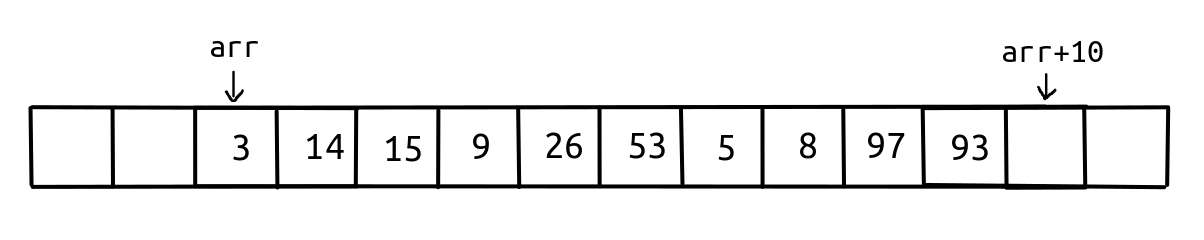
\includegraphics[width=0.9\textwidth]{poglavja/urejanje/addressing}
\end{figure*}

Optimalna časovna zahtevnost algoritma za urejanje je $O(n \log n)$.
To v praksi pomeni, da bo urejanje delovalo dovolj hitro za $n \le 10^6$
podatkov.
Če imamo več podatkov kot toliko, bo urejanje trajalo predolgo in naša rešitev
ne bo sprejeta.

\naslov{Primerjalna funkcija}

Če želimo urediti seznam padajoče namesto naraščajoče, lahko seznam prvo uredimo
naraščajoče, in ga nato obrnemo.
Ker s tem dobimo veliko dodatnega dela, je bolje, da funkciji \koda{sort} podamo
lastno primerjalno funkcijo.
Le-ta mora sprejeti dva argumenta ter vrniti \koda{bool}, in sicer; če mora biti
prvi argument v urejenem seznamu levo od drugega, mora funkcija vrniti \koda{true},
sicer pa \koda{false}.
Če ne podamo tretjega argumenta, se \koda{sort} obnaša tako, kot da bi podali
naslednjo funkcijo:

\fkoda{poglavja/urejanje/compare.cpp}

Če želimo urediti seznam padajoče, moramo torej le podati nasprotno funkcijo,
kot spodaj:

\fkoda{poglavja/urejanje/nasprotno.cpp}

\naslov{Urejanje sestavljenih podatkov}

Recimo, da imamo v nalogi dana imena tekmovalcev ter točke, ki so jih ti
tekmovalci dosegli na tekmovanju, naš cilj pa je, da izpišemo imena tekmovalcev
po vrsti glede na doseženo število točk.
Če bomo prebrali točke in imena v različna seznama, ter uredili seznam točk, bo
seznam imen ostal nespremenjen in ne bomo več vedeli, katero ime pripada katerim
točkam.

Kako uredimo oba seznama hkrati?
Najbolj enostavna možnost je uporaba \koda{struct}, ki pa ga še ne poznamo.
Namesto tega si lahko pripravimo seznam indeksov, ki na začetku na $i$-tem mestu
hrani številko $i$.
Potem sestavimo funkcijo \koda{compare} tako, da sprejme dva indeksa, ter ju uredi
glede na vrednosti v tabeli s točkami na pripadajočih indeksih.
Urejamo pa ne tabele s točkami, temveč novo tabelo indeksov.
Na ta način se tabeli s točkami in z imeni ne bosta spreminjali, in bodo točke
pripadale imenu na istem indeksu.

Primer implementacije opisane rešitve je prikazan spodaj.

\fkoda{poglavja/urejanje/kombinirani.cpp}

\noindent
Če programu podamo spodnji vhod,
\begin{verbatim}
5
France 37
Gregor 34
Julija 38
Matija 29
Urska 8
\end{verbatim}
nam bo izpisal imena, urejena padajoče po številu točk:
\begin{verbatim}
Julija
France
Gregor
Matija
Urska
\end{verbatim}

\poglavje{Hitrost programov in asimptotična notacija}
\naslov{Merjenje hitrosti programa}

Pogosto obstaja več možnosti, kako se lahko lotimo reševanja danega problema.
Če želimo najti najmanjši element v seznamu, lahko na primer pregledamo celoten
seznam in  si beležimo najmanjšega, ki smo ga našli do sedaj, lahko pa celoten
seznam uredimo po vrsti in nato izberemo prvi element.
Pričakujemo lahko, da se bodo različni algoritmi za reševanje istega problema
razlikovali tudi po tem, kako hitro problem rešijo.
Kako pa v računalništvu izmerimo hitrost? Če delamo samo na enem računalniku,
lahko izmerimo, konkretno koliko časa je program potreboval, da je zaključil
z delovanjem.
Na ta način lahko na primerih demonstriramo, da je nek algoritem boljši od
drugega; ko pa želimo naše rezultate deliti in primerjati z drugimi,
pa se ne moramo zanašati, da bodo imeli enako močen računalnik kot mi, in da
bodo njihovi testni primeri primerljivo zahtevni z našimi.
Dejansko so težave pri tem še hujše; na hitrost delovanja našega programa ne
vpliva samo strojna oprema računalnika (torej, kakšen procesor ima, koliko ima
spomina itd.), temveč tudi ostali programi, ki jih imamo hkrati odprte.
Če se želimo pogovarjati o hitrosti algoritmov, potrebujemo bolj abstraktno
orodje.
Na pomoč pride asimptotična zahtevnost.

Da določimo hitrost našega programa, moramo prvo določiti, katere spremenljivke
vplivajo na čas delovanja, ter kako je čas od njih odvisen.
Rezultat take analize zapišemo kot izraz v oklepaje, pred katere zapišemo
veliko črko O, takole: $O(\ldots)$.
Poglejmo si primer.

\fkoda{poglavja/asimptoticna-notacija/poisci-najmanjsega.cpp}

Funkcija \koda{poisci_najmanjsega} sprejme število $n$, ki pove dolžino seznama
\koda{arr}.
Po seznamu se nato enkrat sprehodi, in si ob tem beleži indeks najmanjšega
elementa, ki ga je do sedaj našla.
Razmislimo, katere vse različne operacije zgornji program opravi.
\begin{itemize}
\item 
  Večkrat med programom nastavimo neki spremenljivki novo vrednost.
\item
  V vsaki iteraciji zanke prištejemo 1 spremenljivki \koda{i}.
\item
  Poleg tega v vsaki iteraciji zanke tudi primerjamo \koda{i} z \koda{n},
\item
  dvakrat dostopamo do nekega elementa v seznamu,
\item
  ter ju primerjamo.
\item
  Na koncu še enkrat dostopamo do elementa v seznamu, ter ga vrnemo.
\end{itemize}

Vse naštete operacije same po sebi \emph{trajajo} $O(1)$ časa.
To pomeni, da se vedno izvajajo enako hitro, neodvisno od parametrov, ki jim
podamo (npr.~dve števili bomo vedno enako hitro sešteli, ne glede na to, ali
seštevamo $5 + 7$ ali $123456+984621$).
Rečemo tudi, da porabijo \emph{konstantno mnogo} časa.

Kolikokrat pa izvedemo te operacije?
Analizirajmo najslabši primer za naš program; če je seznam \koda{arr} padajoče
urejen.
Tedaj bomo v vsaki iteraciji zanke enkrat primerjali \koda{i < n}, dvakrat
dostopali do vseh elementov podanega seznama, enkrat primerjali
\koda{arr[min_idx] > arr[i]}, enkrat nastavili \koda{min_idx}, ter enkrat
povečali \koda{i}.
Zunaj zanke bomo nastavili \koda{min_idx} ter \koda{i} na začetni vrednosti, ter
še enkrat dostopali do elementa v seznamu.
Zanka se vedno izvaja za natanko \koda{n} iteracij; vedno vsak element pregledamo
enkrat.
Torej je celotna časovna zahtevnost našega programa $O(3 + 6n)$.
Ker pa za velike $n$ del zunaj zanke hitro postane nepomemben, ga ignoriramo, in
zanemarimo $3$ v časovni zahtevnosti.
Poleg tega ignoriramo tudi faktor $6$ pred členom $n$ -- ker tako in tako ne moramo
vedeti, kako hitre so operacije v zanki v primerjavi druga z drugo, te konstante
ne moramo natančno določiti.
Končna časovna zahtevnost našega programa je torej $O(n)$.

To je tudi najboljši možni algoritem za iskanje najmanjšega elementa v seznamu.
Če bi nek algoritem namreč deloval v hitrejšem času kot $O(n)$, bi moral
nekatera mesta v seznamu izpustiti; če tedaj algoritmu podamo seznam, ki ima
najmanjši element ravno na takem mestu, ga algoritem ne bo našel, in bo podal
napačen odgovor.

Pomembna opazka je, da hitrost našega algoritma ni odvisna od velikosti števil
v seznamu, temveč le od velikosti seznama.
Naslednji program prav tako poišče najmanjše število v seznamu, vendar je
konkretno počasnejši od zgornjega:

\fkoda{poglavja/asimptoticna-notacija/poisci-najmanjsega-slabsi.cpp}

V tem programu imamo dve zanki; ena se sprehaja po vseh možnih vrednosti števil
v seznamu, druga pa preverja, če je ta element dejansko v seznamu.
Vsakič, ko se zunanja zanka izvede enkrat, se notranja izvede \koda{n}-krat (v
najslabšem primeru), zunanja zanka pa se izvede \koda{(m+1)}-krat.
Torej je zahtevnost $O((m+1) \cdot n)$, oziroma $O(mn + n)$.
Člen $n$ v vsoti pa je v vseh primerih manjši od člena $mn$ ali njemu enako
velik, zato ga kot prej izpustimo.
Končna časovna zahtevnost drugega algoritma je torej $O(mn)$.

Spremenljivka tipa \koda{int} lahko hrani števila, velika do približno dve
milijardi -- v najslabšem primeru je $m$ torej približno $2 \cdot 10^9$.
Če prvi algoritem na nekem računalniku potrebuje eno sekundo, da se konča, bi
drugi algoritem v najslabšem primeru na istem računalniku potreboval več kot
šestdeset let.

Poglejmo si še nekaj primerov.
Naslednji program za vsako število v seznamu \koda{arr} poišče število števil
desno od njega, ki so večja.
Notranja zanka se v prvi iteraciji izvede $(n-1)$-krat, v drugi iteraciji
$(n-2)$-krat, v tretji $(n-3)$-krat, itd.
V zadnji iteraciji se sploh ne izvede.
Skupaj se koda znotraj notranje zanke ponovi tolikokrat:
\[
  (n-1) + (n-2) + \ldots + 1 + 0 = \frac{n(n-1)}{2}
\]
Spet ignoriramo konstanto $\frac{1}{2}$ ter člen samo z $n$, in pridemo do
zahtevnosti $O(n^2)$.

\fkoda{poglavja/asimptoticna-notacija/stevilo-vecjih.cpp}

Spodnji program preveri, če je število \koda{n} praštevilo.
Program ima eno zanko, ki se sprehaja toliko časa, dokler kvadrat spremenljivke
$i$ ne postane večji od $n$, oz.~dokler je $i \le \sqrt{n}$.
Zanka se torej izvede v $O(\sqrt{n})$.

% Zahvala Roku Lavriču za popravek v kodi
\fkoda{poglavja/asimptoticna-notacija/prastevilo.cpp}

\naslov{Klasifikacija}

Računalnik lahko v eni sekundi opravi približno $10^7$ operacij.
Da določimo, kako dober algoritem potrebujemo za rešitev neke naloge, lahko
preverimo omejitve vhodnih podatkov.
Spodnja tabela prikazuje nekaj pogostih časovnih zahtevnosti, ter pripadajoče
največje omejitve.
Z uporabo te tabele lahko vnaprej določimo, kakšno največjo časovno zahtevnost
mora imeti naš program, da reši določeno nalogo.

\begin{table}[h!]
  \centering
  \begin{tabular}{|c|c|c|}
	\hline
	Zahtevnost & Omejitev za \(n\) & Ime zahtevnosti \\
	\hline
	$O(1)$ & brez & \emph{konstantna} \\
	$O(\log n)$ & zelo visoka & \emph{logaritemska} \\
	$O(\sqrt{n})$ & $10^{14}$ & \emph{korenska} \\
	$O(n)$ & $10^7$ & \emph{linearna} \\
	$O(n \log n)$ & $10^6$ & \\
	$O(n^2)$ & $10^4$ & \emph{kvadratna} \\
	$O(n^3)$ & $300$ & \emph{kubična} \\
	$O(2^n)$ & $20$ & \emph{eksponentna} \\
	\hline
  \end{tabular}
\end{table}

\end{document}